% ----------------------------------------------------------
% Introdução (exemplo de capítulo sem numeração, mas presente no Sumário)
% ----------------------------------------------------------
\chapter{Introdução}
% ----------------------------------------------------------

A inteligência artificial (IA) vem ganhando manchetes no mundo todo,sendo anunciada tanto como uma salvação econômica quanto como precursora de desintegração social. Quando computadores programáveis foram concebidos pela primeira vez, as pessoas se perguntavam se essas máquinas poderiam se tornar inteligentes, mais de cem anos antes de uma ser construída.
% \cite{menabrea1843sketch}.
 Hoje, a inteligência artificial é um campo com inúmeras aplicações práticas e tópicos de pesquisa ativos. Buscamos softwares inteligentes para automatizar o trabalho de rotina, entender a fala ou as imagens, fazer diagnósticos em medicina e apoiar a pesquisa científica \cite{Goodfellow-et-al-2016}.


A IA adiciona inteligência a produtos existentes. Na maioria dos casos, a inteligência artificial não é vendida como uma aplicação individual. Pelo contrário, produtos já existentes são aprimorados com funcionalidades de IA, de maneira parecida como a Siri foi adicionada aos produtos da \textit{Apple}. Automação, plataformas de conversa, robôs e aparelhos inteligentes podem ser combinados com grandes quantidades de dados para aprimorar diversas tecnologias para casa e escritório, de inteligência em segurança à análise de investimentos.

A maioria dos exemplos de IA sobre os quais se ouve falar hoje – de computadores mestres em xadrez a carros autônomos – dependem de \textit{deep learning} e processamento de linguagem natural (PNL) \cite{pln-o-que-e}. Treinar um agente para superar os jogadores humanos e otimizar sua performance pode nos ensinar como otimizar diferentes processos em uma grande variedade de situações. Foi o que o \textit{DeepMind} do Google fez com seu popular \textit{AlphaGo} e seu sucessor \textit{AlphaZero}, vencendo os campeões mundiais em Go, xadrez e shogi, e obtendo resultados de performance nunca antes vistos.

\section{Motivação}

Técnicas de aprendizado de máquina e algoritmos de \textit{deep learning} têm consistentemente melhorado a capacidade de um computador de fornecer reconhecimento de padrões e previsões cada vez mais precisas. Além disso, sistemas de DL são consistentemente aplicados com sucesso a conjuntos de aplicações cada vez mais amplos.

Ao mesmo tempo em que a escala e a precisão das redes profundas aumentaram, a complexidade das tarefas que podem ser resolvidas também cresceu significativamente. 
Uma conquista importante de sistemas de DL é a sua extensão ao domínio da aprendizagem por reforço (\textit{reinforcement learning}) \cite{reinforcement-learning-intro-2018}. No contexto do aprendizado por reforço, um agente autônomo deve aprender a executar uma tarefa por tentativa e erro, sem nenhuma orientação do operador humano. 

Além do valor para pesquisa em múltiplas áreas da ciência, muitas dessas aplicações de aprendizado de máquina e \textit{deep learning} são altamente lucrativas. O aprendizado de máquina hoje é usado por muitas empresas de tecnologia, incluindo \textit{Google, Microsoft, Facebook}, IBM, \textit{Baidu, Apple, Adobe, Netflix}.

Diante à crescente presença de sistemas que utilizam técnicas de \textit{deep learning} no dia-a-dia, nota-se o grande potencial do investimento em pesquisa, modelagem de novos problemas e estudo de técnicas de aprendizado de máquina. 
%
Uma interessante aplicação desses sistemas está na área de jogos digitais. A indústria de videogames tem testemunhado um enorme crescimento, graças, em boa parte, ao incrível aumento no poder da computação em termos de representações visuais. 
%
%
Seja no controle de personagens não-jogadores (NPC), ou para a geração de conteúdo processual (PCG), são inúmeras as potenciais aplicações dessas técnicas em jogos digitais.
%
O potencial dessas ferramentas de obter uma vantagem competitiva no mercado, ou simplesmente fornecer uma melhor experiência para o usuário é, no mínimo, instigante.
%
Nesse contexto, a modelagem de novos problemas, implementação de soluções utilizando técnicas de \textit{deep learning} e investimento na área, torna-se uma relevante contribuição para o estado da arte.


\section{Objetivos}
 O presente trabalho tem como objetivo propor o desenvolvimento de uma IA capaz de aprender a jogar diferentes jogos, desde que se tenha acesso ao código fonte e feito em Allegro. Para isso, será implementado um algoritmo de \textit{Deep Reinforcement Learning}, abordagem que consiste em fornecer ao sistema parâmetros relacionados ao seu estado e uma recompensa positiva ou negativa com base em suas ações. 
 % Nenhuma regra sobre o jogo é dada e, inicialmente, a IA não tem informações sobre o que precisa fazer. A única informação passada para a IA são os comandos básicos do jogo. 
 O objetivo do sistema é descobrir e elaborar uma estratégia para maximizar a pontuação - ou a recompensa.
 % Diferente de muitas IAs que focam na solução de um único problema, a proposta deste projeto é elaborar uma IA que seja genérica e capaz solucionar e elaborar estratégias para uma variedade de situações diferentes.

 % Os objetivos mais específicos do trabalho são:

 % \begin{enumerate}
 % 	\item Revisão da literatura do projeto;
 % 	\item Proposta de um algoritmo de \textit{deep learning} para a solução do problema;
 % 	\item !!!!!TODO!!!!!
 % \end{enumerate}

\section{Descrição do problema}
O campo inteligência artificial é capaz de solucionar, com certa facilidade, problemas que são intelectualmente muito difíceis para os serem humanos, mas relativamente diretos para os computadores - problemas que podem ser descritos por uma lista de regras formais e matemáticas. Tarefas abstratas e formais que estão entre os empreendimentos mentais mais difíceis para um ser humano estão entre os mais fáceis para um computador.

Ironicamente, o grande desafio à inteligência artificial provou estar em resolver tarefas fáceis de executar para um ser humano. Problemas  que parecem automáticos, que resolvemos intuitivamente, como reconhecer palavras faladas ou rostos em imagens. Os computadores há muito conseguem derrotar até o melhor jogador de xadrez humano \cite{Hsu:2002:BDB:601291}, mas apenas recentemente começaram a combinar algumas das habilidades dos seres humanos comuns em reconhecer objetos ou fala. 

A vida cotidiana de uma pessoa requer uma imensa quantidade de conhecimento sobre o mundo. A grande quantidade de informação desses cenários torna inviável a codificação de todas as regras do sistema e, por isso, o computador tem uma grande dificuldade para solucionar esses problemas. Além disso, grande parte desse conhecimento é subjetivo e intuitivo e, portanto, difícil de articular de maneira formal. Os computadores precisam capturar esse mesmo conhecimento para se comportarem de maneira inteligente. Um dos principais desafios da inteligência artificial é como obter esse conhecimento informal em um computador.

\subsection{\textit{Deep Learning}}

 As dificuldades enfrentadas por sistemas que dependem de conhecimento codificado sugerem que os sistemas de IA necessitam da capacidade de adquirir seu próprio conhecimento, extraindo padrões de dados brutos. Esse recurso é conhecido como aprendizado de máquina ou \textit{machine learning} (ML). A introdução do aprendizado de máquina permitiu que os computadores resolvessem problemas que envolvem o conhecimento sobre o mundo real e tomassem decisões mais subjetivas.

 O \textit{deep learning} (DL) é uma área do aprendizado de máquina que propõe que os computadores aprendam com a experiência, se ajustem à novas entradas de dados e compreendam o mundo em termos de hierarquia de conceitos, sendo cada conceito definido por sua relação com conceitos mais simples. 
 Ao reunir conhecimento a partir da experiência, essa abordagem evita a necessidade dos operadores humanos de especificar formalmente todo o conhecimento que o computador precisa. Além disso, a hierarquia de conceitos permite que o computador aprenda conceitos complexos, construindo-os a partir de conceitos mais simples. Isso nos permite treinar os computadores para cumprir tarefas específicas ao processar grandes quantidades de dados e reconhecer padrões nesses dados.

 A \textbf{Figura \ref{hierarquia-conceitos-dl}} mostra como um sitema de \textit{deep learning} representa o conceito de imagem de uma pessoa combinando conceitos mais simples, como cantos e contornos, que por sua vez são definidos em termos de arestas. 
 O mapeamento de funções de um conjunto de pixels para uma identidade de objeto é muito complicado. O algoritmo de \textit{deep learning} resolve essa dificuldade dividindo o mapeamento complicado desejado em séries de mapeamentos simples aninhados, cada um deles descrito por uma camada diferente do modelo. A entrada é apresentada na camada visível, assim denominada porque contém as variáveis que podemos observar.
 Em seguida, uma série de camadas ocultas extrai recursos cada vez mais abstratos da imagem. Essas camadas são chamadas de "ocultas" porque seus valores não são fornecidos nos dados; em vez disso, o algoritmo deve determinar quais conceitos são úteis para explicar os relacionamentos nos dados observados. A camada de saída obtém a identidade de objeto abstrata a partir dos conceitos obtidos pelas camadas ocultas.


 \begin{figure}[h]
 \centering
 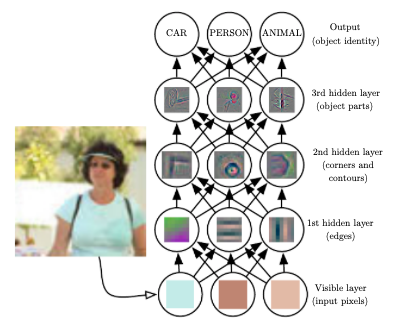
\includegraphics[width=.6 \textwidth]{conteudo/imgs/hierarquia-conceitos-dl.png}
 \caption[Ilustração de um modelo de aprendizado profundo]{Ilustração de um modelo de aprendizado profundo. Dados os pixels, a primeira camada pode identificar facilmente as bordas, comparando o brilho dos pixels vizinhos. Dada a descrição das arestas pela primeira camada oculta, a segunda camada oculta pode procurar facilmente cantos e contornos estendidos, reconhecíveis como coleções de arestas. Dada a descrição da segunda camada oculta da imagem em termos de cantos e contornos, o terceiro setor oculto pode detectar partes inteiras de objetos específicos, encontrando coleções específicas de contornos e cantos. Finalmente, esta descrição da imagem em termos das partes do objeto que ela contém pode ser usada para reconhecer os objetos presentes na imagem. Figura retirada de \cite{Goodfellow-et-al-2016}}
 \label{hierarquia-conceitos-dl}
 	\end{figure}

\section{Revisão da literatura }

No contexto de \textit{reinforcement learning}, o \textit{DeepMind} demonstrou que um aprendizado por reforço, baseado no aprendizado profundo, é capaz de aprender a jogar videogames Atari, atingindo desempenho em nível humano em diversas tarefas \cite{mnih-human-control-drl}.

O \textit{deep learning} também contribuiu para outras ciências. As redes convolucionais modernas para reconhecimento de objetos fornecem um modelo de processamento visual que os neurocientistas podem estudar \cite{dicarlo-afrax-yamins:2014}. O \textit{deep learning} também fornece ferramentas úteis para processar grandes quantidades de dados e fazer previsões úteis em campos científicos. Ele tem sido usado com sucesso para prever como as moléculas irão interagir, a fim de ajudar as empresas farmacêuticas a projetar novos medicamentos \cite{dahl2014multitask}, a procurar partículas subatômicas \cite{baldi:s:w:2015}. Espera-se que o DL apareça em cada vez mais campos científicos no futuro.







